\begin{frame}{Dimension Reduction Methods}{Principal Component Analysis (PCA)}

Let's define what is \textbf{PCA} \pause 

\begin{itemize}
    \item PCA is a technique for reducing the dimension of an $n \times p$ data matrix $X$. \pause 

    \item The \textit{first PC} $(Z_1)$ direction of the data is that along which the observations \textit{vary the most}. \pause  \\
    $\rightarrow$ If we protect the $n$-observations onto this FP direction, then the resulting projected observations would have the largest variance. \pause 

    \item In general, one can construct up to $p$ distinct PC. \pause 
        
    \item The second PC $Z_2$ is a linear combination of the variables that is uncorrelated with $Z_1$ , and has largest variance subject to this constraint. \pause 

    \begin{figure}
        \centering
        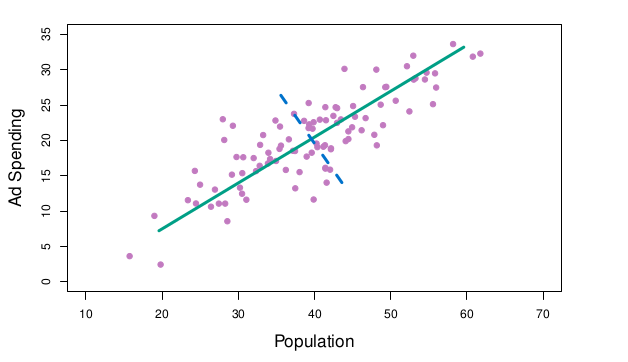
\includegraphics[height=3.5cm]{dim-reduction/pca.png}
    \end{figure} \pause 

\end{itemize}
    
\end{frame}

\begin{frame}{Dimension Reduction Methods}{Principal Component Regression (PCR)}
    \begin{itemize}

    \item The PCR approach involves construct the first $M$ principal components, $Z_1 , \cdots , Z_M $, and then using them as the predictors in a OLS model. \pause 

    \item The key idea is that small number of PC suffice to explain most of the variability in the data, as well the relationship with $Y$. \pause 

    \item In other words, we \textbf{assume} that the directions in which $X_1 , \cdots , X_p$ show the most variation are the directions that are associated with $Y$. \pause 

    \item If the assumption holds, then fitting a OLS model to $Z_1 , \cdots , Z_M $ will lead to better results than fitting a OLS to $X_1 , \cdots , X_p$. \pause 

    \item The number of PC, $M$, is typically chosen by cross-validation. \pause 
    \end{itemize}


    \begin{block}{Note}

    \begin{itemize}
        \item These PC directions are identified in an \textcolor{blue}{unsupervised way}. \pause \\
        $\rightarrow Y$ does not supervise the identification of the PC. \pause 
        \\ 

        \item There is no guarantee that the directions that best explain the predictors will also be the best directions to use for predicting $Y$.
    \end{itemize}
        
    \end{block}
    

    
\end{frame}